\documentclass[8pt,twocolumn]{article}
%\usepackage{amsmath,amssymb,amsthm,amsbsy,amsfonts,mathtools}
\usepackage{amsmath}
\usepackage{amssymb}
\usepackage{amsthm}
\usepackage{physics}
\usepackage{hyperref}
\usepackage{exercise}
\usepackage[makeroom]{cancel}
\usepackage[margin=2em]{geometry}

\usepackage{graphicx}

\usepackage{footmisc}
\DefineFNsymbols{mySymbols}{{\ensuremath\dagger}{\ensuremath\ddagger}\S\P
   *{**}{\ensuremath{\dagger\dagger}}{\ensuremath{\ddagger\ddagger}}}
\setfnsymbol{mySymbols}

\newcommand{\N}{\mathbb{N}}
\newcommand{\R}{\mathbb{R}}
\newcommand{\Z}{\mathbb{Z}}
\newcommand{\Q}{\mathbb{Q}}

\newenvironment{theorem}[2][Theorem]{\begin{trivlist}
\item[\hskip \labelsep {\bfseries #1}\hskip \labelsep {\bfseries #2.}]}{\end{trivlist}}
\newenvironment{lemma}[2][Lemma]{\begin{trivlist}
\item[\hskip \labelsep {\bfseries #1}\hskip \labelsep {\bfseries #2.}]}{\end{trivlist}}
\newenvironment{exercise}[2][Exercise]{\begin{trivlist}
\item[\hskip \labelsep {\bfseries #1}\hskip \labelsep {\bfseries #2.}]}{\end{trivlist}}
\newenvironment{problem}[2][Problem]{\begin{trivlist}
\item[\hskip \labelsep {\bfseries #1}\hskip \labelsep {\bfseries #2.}]}{\end{trivlist}}
\newenvironment{question}[2][Question]{\begin{trivlist}
\item[\hskip \labelsep {\bfseries #1}\hskip \labelsep {\bfseries #2.}]}{\end{trivlist}}
\newenvironment{corollary}[2][Corollary]{\begin{trivlist}
\item[\hskip \labelsep {\bfseries #1}\hskip \labelsep {\bfseries #2.}]}{\end{trivlist}}
\newenvironment{answer}[2][Answer]{\begin{trivlist}
\item[\hskip \labelsep {\bfseries #1}\hskip \labelsep {\bfseries #2.}]}{\end{trivlist}}

\let\emph\relax % there's no \RedeclareTextFontCommand
\DeclareTextFontCommand{\emph}{\bfseries\em}

\setlength{\columnseprule}{0.4pt}
\setlength{\columnsep}{3em}

\usepackage{todonotes}

\author{Yingbo Ma \thanks{Student ID: \tt{16058474}}}
\title{\vspace{-1.cm}Homework 5}
\date{May 15, 2018}

\begin{document}
\maketitle

\begin{Answer}[number=29]
  \emph{16.1.29:}
  The function $f(x,y) = x^2 + y^2$ has the gradient $\grad f(x,y) =
  \mqty[2x\\2y]$. All the vectors point away from the origin.
  Thus $\grad f$ corresponds to graph \RC3.

  \emph{16.1.30:}
  The function $f(x,y) = x(x+y)$ has the gradient $\grad f(x,y) =
  \mqty[2x+y\\x]$. The vectors point upward when $x>0$, and vectors point
  downward when $x<0$.
  Thus $\grad f$ corresponds to graph \RC4.

  \emph{16.1.31:}
  The function $f(x,y) = (x+y)^2$ has the gradient $\grad f(x,y) =
  \mqty[2x+2y\\2x+2y]$. The vectors vanish along the line $y=-x$.
  Thus $\grad f$ corresponds to graph \RC2.

  \emph{16.1.32:}
  The function $f(x,y) = \sin \sqrt{x^2+y^2}$ has the gradient $\grad f(x,y) =
  \frac{\cos\sqrt{x^2+y^2}}{\sqrt{x^2+y^2}}\mqty[x\\y]$. The magnitude of
  vectors changes periodically as its distance grows from the origin.
  Thus $\grad f$ corresponds to graph \RC1.

  \emph{16.2.17:}
  The function $\bm{F}$ have positive $y$-component along the line $x=-3$, and
  since the path goes upward, the integrand of the integral
  $\int_{C_1}\bm{F}\cdot \dd{\bm{r}} = \int_{C_1}\bm{F}\cdot\bm{T} \dd{s}$ always
  stay positive, thus the line integral is also positive.

  \emph{16.2.8:}
  Let $C = C1 + C2$ and we have $C_1: x=2\cos t, y=2\sin t, 0\le t \le
  \frac{pi}{2}$ and $C_2: x=4t, y=t+2, 0\le t\le 1$. We then have the integral
  \begin{align*}
    \int_C x^2\dd{x}+y^2\dd{y} &= \int_{C_1} x^2\dd{x}+y^2\dd{y} + \int_{C_2}
    x^2\dd{x}+y^2\dd{y} \\
    &= \int_0^{\frac{\pi}{2}}(2\cos t)^2 (-2\sin t\dd{t}) \\
    &+ (2\sin t)^2 (2\cos t\dd{t}) + \int_0^1 (4t)^2 4\dd{t} + (t+2)^2 \dd{t}
    \\
    &= \int_0^{\frac{\pi}{2}}8 (\sin^2 t \cos t - \cos^2 t\sin t)\dd{t} \\
    &+\int_0^1 65t^2+4t+4 \dd{t}
  \end{align*}
\end{Answer}

\begin{Answer}[number=30]
  Let $f(x,y)=x^2y$ and let $\bm{F}(x,y)=\grad f(x,y) = \mqty[2xy\\ x^2]$. We
  have $C_1: x=2t, y=4t, 0\le t\le 1$ and $C_2: x=2t, y=4t^2, 0\le t\le 1$. We
  have
  \begin{align*}
    \int_{C_1} \bm{F}\cdot \dd{\bm{r}} &= \int_{C_1} 2xy \dd{x} + x^2\dd{y} \\
    &= \int_0^1 2(2t)(4t) 2\dd{t} + (4t)^2 4\dd{t} = 16\int_0^1 3t^2\dd{t} \\
    &=16 \eval{t^3}_0^1 = 16
  \end{align*}
  and
  \begin{align*}
    \int_{C_2} \bm{F}\cdot \dd{\bm{r}} &= \int_{C_2} 2xy \dd{x} + x^2\dd{y} \\
    &= \int_0^1 2(2t)(4t^2) 2\dd{t} + (2t^2)^2 8t\dd{t} = \int_0^1 32t^3 + 32t^3\dd{t} \\
    &= 16\int_0^1 4t^3 \dd{t} = 16 \eval{t^4}_0^1 = 18.
  \end{align*}
  Thus, \(\int_{C_2} \bm{F}\cdot \dd{\bm{r}}\) and \(\int_{C_1} \bm{F}\cdot
  \dd{\bm{r}}\) have the same value.
\end{Answer}

\begin{Answer}[number=31]
  \begin{itemize}
    \item
    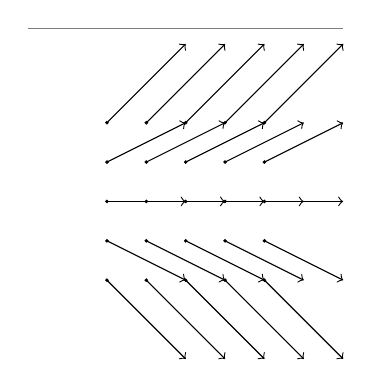
\begin{tikzpicture}
      \draw[step=0.2cm, thin,color=gray] (-2,2) grid (2,2);
        \foreach \x in {-1, -0.5, 0, 0.5, 1} {
          \foreach \y in {-1, -0.5, 0, 0.5, 1} {
              \node at (\x, \y)[circle, fill=black, scale=0.15] {};
              \pgfmathsetmacro{\vx}{1}
              \pgfmathsetmacro{\vy}{\y}
              \draw[->] (\x,\y) -- (\x+\vx, \y+\vy);
          }
      }
      \end{tikzpicture}
      \item
        Such parametric equation can be $C: (x,y)=(t, \frac{t^2}{2})$ which has the
        tangent vector $\mqty[1\\ t_0]$ at $t_0$, which is parallel to the
        vector field $\eval{\bm{F}(x,y)}_{t_0}=\mqty[1\\t_0]$.
  \end{itemize}
\end{Answer}

\end{document}
